% Created 2023-08-26 Sat 18:19
% Intended LaTeX compiler: pdflatex
\documentclass[11pt]{article}
\usepackage[utf8]{inputenc}
\usepackage[T1]{fontenc}
\usepackage{graphicx}
\usepackage{longtable}
\usepackage{wrapfig}
\usepackage{rotating}
\usepackage[normalem]{ulem}
\usepackage{amsmath}
\usepackage{amssymb}
\usepackage{capt-of}
\usepackage{hyperref}
\usepackage{siunitx, array, tikz}
\usetikzlibrary{angles, calc, quotes}
\author{Hankertrix}
\date{\today}
\title{Kinematics Lecture Notes}
\hypersetup{
 pdfauthor={Hankertrix},
 pdftitle={Kinematics Lecture Notes},
 pdfkeywords={},
 pdfsubject={},
 pdfcreator={Emacs 29.1 (Org mode 9.6.6)}, 
 pdflang={English}}
\begin{document}

\maketitle
\setcounter{tocdepth}{2}
\tableofcontents

\newpage

\section{\(\text{Syst\`eme}\) Internationale (SI) \(\text{d'unit\'es}\) (not very important)}
\label{sec:org50ab051}

This section is just some background on the redefinition of the SI units, which isn't very important, but it is good to know.

\begin{itemize}
\item The metric system was originally conceived as a system of measurement that was \textbf{derivable} from unchanging phenomena.
\item Practical limitations necessitated the use of artefacts - the prototype metre and prototype kilogram. Some were difficult to precisely realise in a laboratory, such as the kelvin, which was defined in terms of the triple point of water.
\item Masses of the prototype kilogram and its secondary copies have shown small variations relative to each other over time.
\item As such, they are not thought to be adequate for the increasing accuracy demanded by science, prompting a search for a suitable replacement.
\end{itemize}


\subsection{Mass drift problem of the old SI}
\label{sec:orgef902c9}

\subsubsection{Mass drift of the prototype kilogram and derivatives}
\label{sec:orga62eb5d}
Masses of the prototype kilogram and its secondary copies have shown small variations relative to each other over time, prompting a search for a suitable replacement.

\subsection{Mass and its relation to fundamental constants}
\label{sec:orgac7b10e}

\begin{itemize}
\item Before 2019, Planck's constant \(h\) had some uncertainty because it is determined experimentally. Frequency \(f\) (or the SI unit for time) and the speed of light \(c\) were already exact by 2019.
\item In contrast, the IPK mass was absolutely certain because by definition it is \(\qty{1}{kg}\).
\item But this kilogram artefact (IPK) is practically inaccessible, being sealed in a vacuum jar and stored in a basement vault in Paris, and there are mass drifts with its derivative artefacts.
\end{itemize}

Thus, the solution was to define Planck's constant to be exact, and the mass of the kilogram will follow. The IPK will no longer be exactly \(\qty{1}{kg}\).


\subsection{Redefinition of SI}
\label{sec:org6cc8914}

\subsubsection{Precedence for change}
\label{sec:org2b94e54}
\begin{itemize}
\item \textbf{1960}: Redefined the SI metre in terms of the wavelength of krypton-86 radiation and discarded the pre-SI metre bar, which was a physical artefact.
\item \textbf{1967}: Redefined the original definition of the second, which was based on Earth's average rotation from 1750 to 1892, with a definition based on the frequency of the radiation emitted or absorbed with a caesium-133 atomic transition between two hyperfine levels of the ground state.
\item \textbf{1983}: Redefined the 1960 definition of the metre with one based on the second, by giving an exact definition of the speed of light in units of metres per second.
\end{itemize}

\subsubsection{Redefinition of SI (2019)}
\label{sec:org88b1483}
There was a fundamental change to the definition of SI units in 2019. SI units became \emph{entirely} derivable from natural phenomena and didn't rely on physical artefacts. Most units were based on fundamental physical constants.

\newpage

\subsubsection{Defining the physical constants}
\label{sec:org22a2e03}
The International Bureau for Weights and Measures proposed that 4 further constants of nature (the first 4 below) be defined to have exact values.

\begin{itemize}
\item \textbf{Planck constant} \(h\) is exactly \(6.62607015 \times 10^{-34}\) joule-second (\(\si{J} \cdot \si{s}\))
\item \textbf{Elementary charge} \(e\) is exactly \(1.602176634 \times 10^{-19}\) coulomb (\(\si{C}\)).
\item \textbf{Boltzmann constant} \(k\) is exactly \(1.380649 \times 10^{-23}\) joule per kelvin (\(\si{J} \cdot \si{K}^{-1}\)).
\item \textbf{Avogadro constant} \(N_A\) is exactly \(6.02214076 \times 10^{23}\) reciprocal mole (\(\si{mol}^{-1}\)).
\item \textbf{Speed of light} \(c\) is exactly 299792458 metres per second (\(\si{m} \cdot \si{s}^{-1}\)).
\item \textbf{Ground state hyperfine structure transition frequency} of caesium-133 atom \(\Delta v_{Cs}\) is exactly 9192631770 hertz (\(\si{\hertz}\)).
\item \textbf{Luminous efficacy} \(K_{cd}\) of monochromatic radiation of frequency \(540 \times 10^{12} \si{\hertz}\) (540 \(\si{\tera\hertz}\)) – a frequency of green-coloured light at approximately the peak sensitivity of the human eye – is exactly 683 lumens per watt (\(\si{lm} \cdot \si{\watt}^{-1}\)).

\newpage
\end{itemize}

\section{Models in physics (also not very important)}
\label{sec:org0f54ed3}

\subsection{Models in physics as maps of the terrain (physical world)}
\label{sec:org19f7cb0}
Consider the legend of Galileo’s experiments on falling objects. He is supposed to have dropped them from the Leaning Tower of Pisa in Italy.
\\[0pt]

"Galileo’s pupil, Vincenzo Viviani, wrote in 1717 in Racconto istorico della vita di Galileo Galilei, p. 606: [\ldots{}dimostrando ciò con replicate esperienze, fatte dall'altezza del Campanile di Pisa con l'intervento delli altri lettori e filosofi e di tutta la scolaresca\ldots{} \textbf{[\ldots{} Galileo showed this [all bodies, whatever their weights, fall with equal speeds] by repeated experiments made from the height of the Leaning Tower of Pisa in the presence of other professors and all the students\ldots{}]."}
\\[0pt]

If Galileo had compared the motion of a rock and a feather, but had not “idealised” the motion, by perhaps imagining that the air could slow down the feather more than the rock, he would not have made the conclusion.
\\[0pt]

It is through an idealisation or model of reality – by creating a map of the terrain – where air resistance is absent or equal for both objects, that Galileo could construct a model that captured the essence of the motion without all the complications of reality.
\\[0pt]

To simplify the analysis of a baseball in flight, we use an idealised model. A real baseball in flight will spin and has a complex shape (a baseball in flight is not completely round). It will also have air resistance and wind that will exert forces on the ball The gravitational force exerted on the ball also depends on the ball's altitude as well.
\\[0pt]

However, the idealised model that we use in physics treats the baseball as a point object (a particle of sorts). We ignore air resistance and we assume the gravitational force exerted on the ball is constant.

\newpage

\subsection{Physics is an empirical science}
\label{sec:org8018d46}
Physics, like chemistry and biology, is an \textbf{empirical} science.
\\[0pt]

It contains propositions in the theories which are not deducible from definitions and must be tested with \textbf{empirical} evidence from observations about nature. At the same time, physics is a \emph{dialogue} with nature and observations can lead to new theory, and vice versa.

Below is a quote from scientific American, "Theoretical Physics Is Pointless without Experimental Tests":
\\[0pt]

\emph{“The experience of subjecting a theoretical conjecture to an experimental test is humbling. If the conjecture turns out to be wrong, it must be adjusted. Becoming a physicist brings with it the privilege of retaining your childhood curiosity throughout your adult life. There is no need to pretend you know more than you actually do, and you can admit mistakes if proven wrong by experience, just like a child who is seeking to learn about the world. Doing pure theory without worrying about experimental verification actually deprives one from the pleasure of learning something new about nature.”}


\section{Kinematics}
\label{sec:orga4e4929}

\subsection{Scalar quantities}
\label{sec:org03df333}
Scalar quantities are physical quantities that only have a magnitude and no direction. Examples of scalar quantities include time (\(\si{s}\)), speed (\(\si{ms^{-1}}\)) and temperature (\(\si{\celsius}\)).

\subsection{Vector quantities}
\label{sec:org173dc48}
Vector quantities are physical quantities that have \textbf{both} a magnitude and a direction. Examples of vector quantities include velocity (\(\si{ms^{-1}}\)), acceleration (\(\si{ms^{-2}}\)) and force (\(\si{N}\)).

\subsection{Position, displacement and distance}
\label{sec:orgd86a2fd}

\subsubsection{Position and coordinate system}
\label{sec:orgdf99316}
To study the motion of an object, we need to specify its \textbf{position} in a coordinate system. In 3D space, the coordinates will be a trio of numbers \((x, y, z)\) for the Cartesian system.

\subsubsection{Displacement (vector quantity)}
\label{sec:org47f5f14}
Displacement is the change in position of an object over a time interval (\(\Delta \vec{x}\)). It is expressed using the equation below, where \(\Delta \vec{x}\) is the displacement of the object, and \(\vec{x_f}\) and \(\vec{x_i}\) are the final position and the initial position of the object respectively:

\[\Delta \vec{x} = \vec{x}_f - \vec{x}_i\]

The displacement is only concerned with the \textbf{end points}, and not the path taken by the object during the time interval.
\\[0pt]

Do note that a change in any physical quantity is always its \textbf{final} value minus its \textbf{initial} value.

\subsubsection{Distance (scalar quantity)}
\label{sec:org47ed39a}
The distance is the length of the entire path taken by an object.


\subsection{Velocity and speed (SI units: \(\si{ms^{-1}}\))}
\label{sec:orga74b472}

\subsubsection{Average velocity (vector quantity)}
\label{sec:org1fc9df9}
The average velocity is the change in an object's position (\(\Delta \vec{x}\)) over a finite time interval (\(\Delta t\)). It is given by the equation below:

\[\text{Average velocity: } \Delta \vec{v}_{av} = \frac{\Delta \vec{x}}{\Delta t} = \frac{\vec{x}_2 - \vec{x}_1}{t_2 - t_1}\]

\subsubsection{Instantaneous velocity (vector quantity)}
\label{sec:org115e682}
The instantaneous velocity is the velocity of an object at a specific instance of time. Mathematically, it is when the limit of the time interval becomes an infinitesimally small value. This is expressed mathematically in the equation below:

\[\text{Instantaneous velocity: } \vec{v} = \lim_{\Delta t \rightarrow 0} \frac{\Delta \vec{x}}{\Delta t} = \frac{d \vec{x}}{dt}\]

In GCE A-level texts, the instantaneous velocity is often defined to be the rate of change of displacement. However, this should not be the case and the instantaneous velocity should be defined as the rate of change of \textbf{position}.

\subsubsection{Speed (scalar quantity)}
\label{sec:org77fb81c}
Speed is defined as the \textbf{magnitude} of velocity.

\subsubsection{Finding velocity from a graph}
\label{sec:org76e28b6}
From the equation for instantaneous velocity above, we know that \(\vec{v} = \frac{d \vec{x}}{dt}\). This means that the gradient at a point of a position-time (\(x - t\)) graph will give the instantaneous velocity of an object at that point in time.


\subsection{Acceleration (SI units: \(\si{ms^{-2}}\))}
\label{sec:orgfcd9159}

\subsubsection{Average acceleration (vector quantity)}
\label{sec:orgf4588b1}
The average acceleration is the change in velocity over a finite time interval. This is expressed mathematically in the equation below:

\[\text{Average acceleration: } \vec{a}_{av} = \frac{\Delta \vec{v}}{\Delta t} = \frac{\vec{v}_2 - \vec{v}_1}{t_2 - t_1}\]

\subsubsection{Instantaneous acceleration (vector quantity)}
\label{sec:org1fff232}
The instantaneous acceleration is the acceleration of an object at a specific instance of time. Mathematically, it is when the limit of the time interval becomes an infinitesimally small value. This is expressed mathematically in the equation below:

\[\text{Instantaneous acceleration: } \vec{a} = \lim_{\Delta t \rightarrow 0} \frac{\Delta \vec{v}}{\Delta t} = \frac{d \vec{v}}{dt} = \frac{d^2 \vec{x}}{dt^2}\]

The units of acceleration give a sense of how to understand this quantity. It is given by metres per second per second, i.e. it is the change in velocity (\(\si{ms^{-1}}\)) every second.

\subsubsection{Finding the acceleration from a graph}
\label{sec:org63b3367}
From the equation for instantaneous acceleration above, we know that \(\vec{a} = \frac{d \vec{v}}{dt}\). This means that the gradient at a point of a velocity-time (\(v - t\)) graph will give the instantaneous velocity of an object at that point in time.

\subsubsection{Accelerating while maintaining a constant speed?}
\label{sec:orga23889c}
Even when the speed of an object is constant (remember that the speed of an object is a scalar quantity), as long as the direction of the object changes, the \textbf{velocity} of the object is \textbf{changing}. This means a car has a non-zero acceleration if it rounds a bend at constant speed. Since the car's direction is changing, its \textbf{velocity} is also \textbf{changing} and hence it has \textbf{non-zero acceleration}.
\\[0pt]

Hence, you should not use the layman understanding of acceleration to mean speeding up. When there is an acceleration, it just means that the velocity is changing, which doesn't necessarily mean that the speed is changing.


\subsubsection{Relating acceleration to velocity}
\label{sec:org6d8c582}

\begin{center}
\begin{tabular}{ |m{11em}|m{11em}| }
\hline
If $x$-velocity is: & $x$-accleration is: \\
\hline
Positive \& increasing (getting more positive) & Positive: The object is moving in the $+ \, x$-direction \& speeding up \\
\hline
Positive \& decreasing (getting less positive) & Negative: The object is moving in the $+ \, x$-direction \& slowing down \\
\hline
Negative \& increasing (getting less negative) & Positive: The object is moving in the $- \, x$-direction \& slowing down \\
\hline
Negative \& decreasing (getting more negative) & Negative: The object is moving in the $- \, x$-direction \& speeding up \\
\hline
\end{tabular}
\end{center}


\subsection{The coordinate system}
\label{sec:orgd38fdd0}
The coordinate system is arbitrary, so the direction of motion of an object can either be considered positive or negative.
\\[0pt]

Usually, an object that is moving upwards will be considered as moving in the \(+ \, y\)-direction while an object that is moving downwards will be considered as moving in the \(- \, y\)-direction.
\\[0pt]

Similarly, an object moving right will usually be considered as moving in the \(+ \, x\)-direction while an object moving left will usually be considered as moving in the \(- \, x\)-direction.


\subsection{Deriving the equations of motion for constant acceleration}
\label{sec:orgb6ff998}
Let the initial time be 0 and the final time be \(t\), i.e. \(t_i = 0, t_f = t\). Let \(v_f\) be the final velocity of an object and \(v_i\) be the initial velocity of an object.
\\[0pt]

The change in velocity would be:
\[v_f - v_i = \int_0^t a \, dt\]

Since acceleration is constant:
\[v_f - v_i = at\]
\[v_f = v_i + at\]

Since the initial velocity is a constant (\(v_0\)) and the final velocity can be expressed as a function of time (\(v(t)\)), we have the \textbf{first} equation of motion:
\[v(t) = v_0 + at \tag{1}\]

With this equation we can also derive the displacement of an object:
\[x_f - x_i = \int_0^t v(t) \, dt\]
\[x_f - x_i = \int_0^t (v_0 + at) \, dt\]
\[x_f - x_i = v_0t + \frac{1}{2}at^2\]

Since the initial displacement is a constant (\(x_0\)) and the final displacement can be expressed as a function of time (\(x(t)\)):
\[x(t) - x_0 = v_0t + \frac{1}{2}at^2\]

Letting \(s\) be the change in displacement, i.e. \(s = x(t) - x_0\), we have the \textbf{second} equation of motion:
\[s = v_0t + \frac{1}{2}at^2 \tag{2}\]

We can arrive at a final, independent equation of motion by using a chain-rule trick:
\[\text{Acceleration } a = \frac{dv}{dt} = \frac{dv}{dx} \frac{dx}{dt}\]
\[a = v \frac{dv}{dx}\]

Integrating with respect to \(x\):
\[\int_{x_i}^{x_f} a \, dx = \int_{v_i}^{v_f} v \, dv\]

Since acceleration is constant:
\[a \int_{x_i}^{x_f} \, dx = \int_{v_i}^{v_f} v \, dv\]
\[a(x_f - x_i) = \frac{1}{2}((v_f)^2 - (v_i)^2)\]
\[2a(x_f - x_i) = (v_f)^2 - (v_i)^2 \tag{a}\]

Since \(x_i\) and \(v_i\) is constant, we can substitute \(x_i = x_0\) and \(v_i = v_0\) into equation \((a)\):
\[2a(x_f - x_0) = (v_f)^2 - (v_0)^2\]
\[(v_f)^2 = (v_0)^2 + 2a(x_f - x_0)\]

Representing \(x_f\) as \(x\), \(v_f\) as \(v\):
\[v^2 = (v_0)^2 + 2a(x - x_0)\]

Representing \(x - x_0\) as \(s\), we get the \textbf{third and final} equation of motion:
\[v^2 = (v_0)^2 + 2as \tag{3}\]

\newpage

\subsection{Resolving vectors}
\label{sec:orgbdd563c}
A vector can be resolved into 2 separate perpendicular vectors that are independent of each other.

\subsubsection{Examples}
\label{sec:org5be6e8c}

\begin{center}
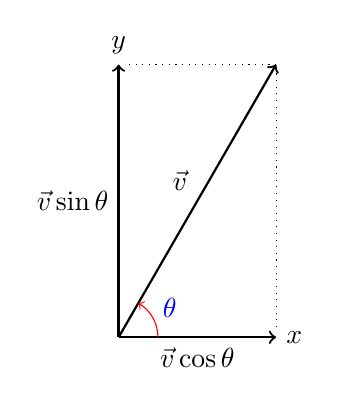
\begin{tikzpicture}

% Start of the 1st example
% Setting the origin
\coordinate (origin) at (0,0);

% Draw the original vector
\draw[thick, ->] (origin) -- ++(60:4) coordinate (vec) node[midway, above left] {$\vec{v}$};

% Draw the resolved vectors
\draw[thick, black, ->] (origin) -- ++(2,0) node (x) {} node[right] {$x$} node[midway, below] {$\vec{v} \cos \theta$};
\draw[thick, black, ->] (origin) -- ++(0,3.464101615) node (y) {} node[above] {$y$} node[midway, left] {$\vec{v} \sin \theta$};

% Draw the dotted lines
\draw[dotted, black] (y) -- ++(2,0);
\draw[dotted, black] (x) -- ++(0,3.464101615);

% Draw the angle
\pic [draw=red, text=blue, ->, "$\theta$", angle eccentricity=1.5] {angle = x--origin--vec};

\end{tikzpicture}
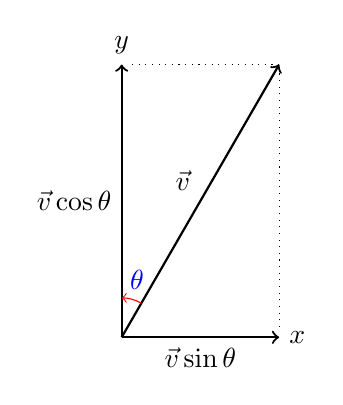
\begin{tikzpicture}

% Start of the 2nd example
% Setting the origin
\coordinate (origin) at (0,0);

% Draw the original vector
\draw[thick, ->] (origin) -- ++(60:4) coordinate (vec) node[midway, above left] {$\vec{v}$};

% Draw the resolved vectors
\draw[thick, black, ->] (origin) -- ++(2,0) node (x) {} node[right] {$x$} node[midway, below] {$\vec{v} \sin \theta$};
\draw[thick, black, ->] (origin) -- ++(0,3.464101615) node (y) {} node[above] {$y$} node[midway, left] {$\vec{v} \cos \theta$};

% Draw the dotted lines
\draw[dotted, black] (y) -- ++(2,0);
\draw[dotted, black] (x) -- ++(0,3.464101615);

% Draw the angle
\pic [draw=red, text=blue, ->, "$\theta$", angle eccentricity=1.5] {angle = vec--origin--y};

\end{tikzpicture}

\[\]

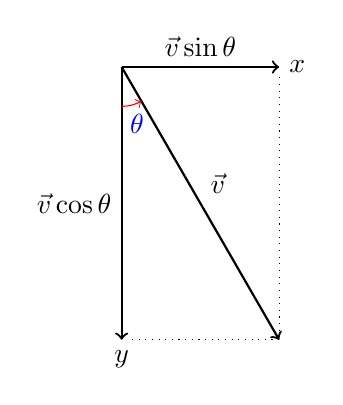
\begin{tikzpicture}

% Start of the 3rd example
% Setting the origin
\coordinate (origin) at (0,0);

% Draw the original vector
\draw[thick, ->] (origin) -- ++(300:4) coordinate (vec) node[midway, above right] {$\vec{v}$};

% Draw the resolved vectors
\draw[thick, black, ->] (origin) -- ++(2,0) node (x) {} node[right] {$x$} node[midway, above] {$\vec{v} \sin \theta$};
\draw[thick, black, ->] (origin) -- ++(0,-3.464101615) node (y) {} node[below] {$y$} node[midway, left] {$\vec{v} \cos \theta$};

% Draw the dotted lines
\draw[dotted, black] (y) -- ++(2,0);
\draw[dotted, black] (x) -- ++(0,-3.464101615);

% Draw the angle
\pic [draw=red, text=blue, ->, "$\theta$", angle eccentricity=1.5] {angle = y--origin--vec};

\end{tikzpicture}
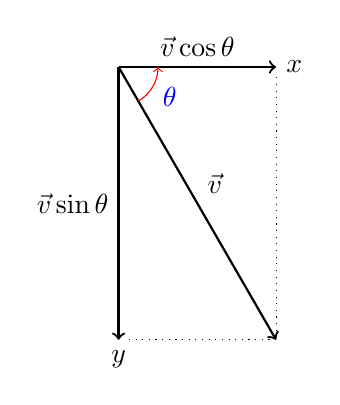
\begin{tikzpicture}

% Start of the 4th example
% Setting the origin
\coordinate (origin) at (0,0);

% Draw the original vector
\draw[thick, ->] (origin) -- ++(300:4) coordinate (vec) node[midway, above right] {$\vec{v}$};

% Draw the resolved vectors
\draw[thick, black, ->] (origin) -- ++(2,0) node (x) {} node[right] {$x$} node[midway, above] {$\vec{v} \cos \theta$};
\draw[thick, black, ->] (origin) -- ++(0,-3.464101615) node (y) {} node[below] {$y$} node[midway, left] {$\vec{v} \sin \theta$};

% Draw the dotted lines
\draw[dotted, black] (y) -- ++(2,0);
\draw[dotted, black] (x) -- ++(0,-3.464101615);

% Draw the angle
\pic [draw=red, text=blue, ->, "$\theta$", angle eccentricity=1.5] {angle = vec--origin--x};

\end{tikzpicture}

\end{center}


In general, the resolved vector \(\vec{v}_r\) that encloses the angle between the original vector \(\vec{v}\) and the resolved vector \(\vec{v}_r\) will have a magnitude of \(\vec{v} \cos \theta\). The other resolved vector will have a magnitude of \(\vec{v} \sin \theta\).

\newpage

\subsection{Relative velocity}
\label{sec:org04cb856}

\subsubsection{Definition}
\label{sec:orga77facd}
The velocity of a moving body seen by a particular observer is called the velocity \emph{relative} to that observer.

\subsubsection{Frame of reference}
\label{sec:org22351c5}
A frame of reference is a coordinate system plus a timescale.

\subsubsection{Conventions}
\label{sec:orgd5d82de}
\begin{itemize}
\item If point \(P\) is moving relative to reference frame \(A\), we denote the velocity of \(P\) relative to frame \(A\) as \(v_{PA}\).
\item If \(P\) is moving relative to frame \(B\) and frame \(B\) is moving relative to frame \(A\), then the velocity of \(P\) relative to frame \(A\) is:
\end{itemize}
\[\vec{v}_{PA} = \vec{v}_{PB} + \vec{v}_{BA}\]

\begin{itemize}
\item Sometimes, it can be helpful to change the sign of the second term together with the subscripts (this doesn't change the equation):
\end{itemize}
\[\vec{v}_{PA} = \vec{v}_{PB} - \vec{v}_{AB},\ \ \because \ \vec{v}_{AB} = -\vec{v}_{BA}\]

Note that \(\because\) means because.

\newpage


\section{Summary}
\label{sec:org3558a35}

\subsection{General relations in kinematics}
\label{sec:org4ab3b16}
\(\indent\) The gradient of a position-time (\(x-t\)) graph is velocity.
\[\vec{v} = \lim_{\Delta t \rightarrow 0} \frac{\Delta \vec{x}}{\Delta t} = \frac{d \vec{x}}{dt}\]

\[\Downarrow\]

The area under a velocity-time (\(v-t\)) graph is displacement.
\[\int_{\vec{x}_i}^{\vec{x}_f} \, d \vec{x} = \int_{t_i}^{t_f} \vec{v} t \, dt\]
\[\vec{x}_f - \vec{x}_i = \int_{t_i}^{t_f} \vec{v} t \, dt\]
\\[0pt]

The gradient of a velocity-time (\(v-t\)) graph is acceleration.
\[\vec{a} = \lim_{\Delta t \rightarrow 0} \frac{\Delta \vec{v}}{\Delta t} = \frac{d \vec{v}}{dt} = \frac{d^2 \vec{x}}{dt^2}\]

\[\Downarrow\]

The area under an acceleration-time (\(a-t\)) graph is acceleration.
\[\int_{\vec{v}_i}^{\vec{v}_f} \, d \vec{v} = \int_{t_i}^{t_f} \vec{a} t \, dt\]
\[\vec{v}_f - \vec{v}_i = \int_{t_i}^{t_f} \vec{a} t \, dt\]


\subsection{Equations of motion for constant acceleration}
\label{sec:orgb7790e2}

\[v = v_0 + at \tag{1}\]
\[s = v_0t + \frac{1}{2} at^2 \tag{2}\]
\[v^2 = {v_0}^2 + 2as \tag{3}\]

\subsection{Relative velocity}
\label{sec:org4c25b6e}
\[\vec{v}_{PA} = \vec{v}_{PB} + \vec{v}_{BA}\]
\end{document}